\section{Функциональные требования}
\label{sec:freq}

Основываясь на требованиях изложенных в разделе \ref{sec:domain:requirements} и диаграмме вариантов использования разработана спецификация требований к разрабатываемому ПС.

\begin{figure}[p]
\centering
    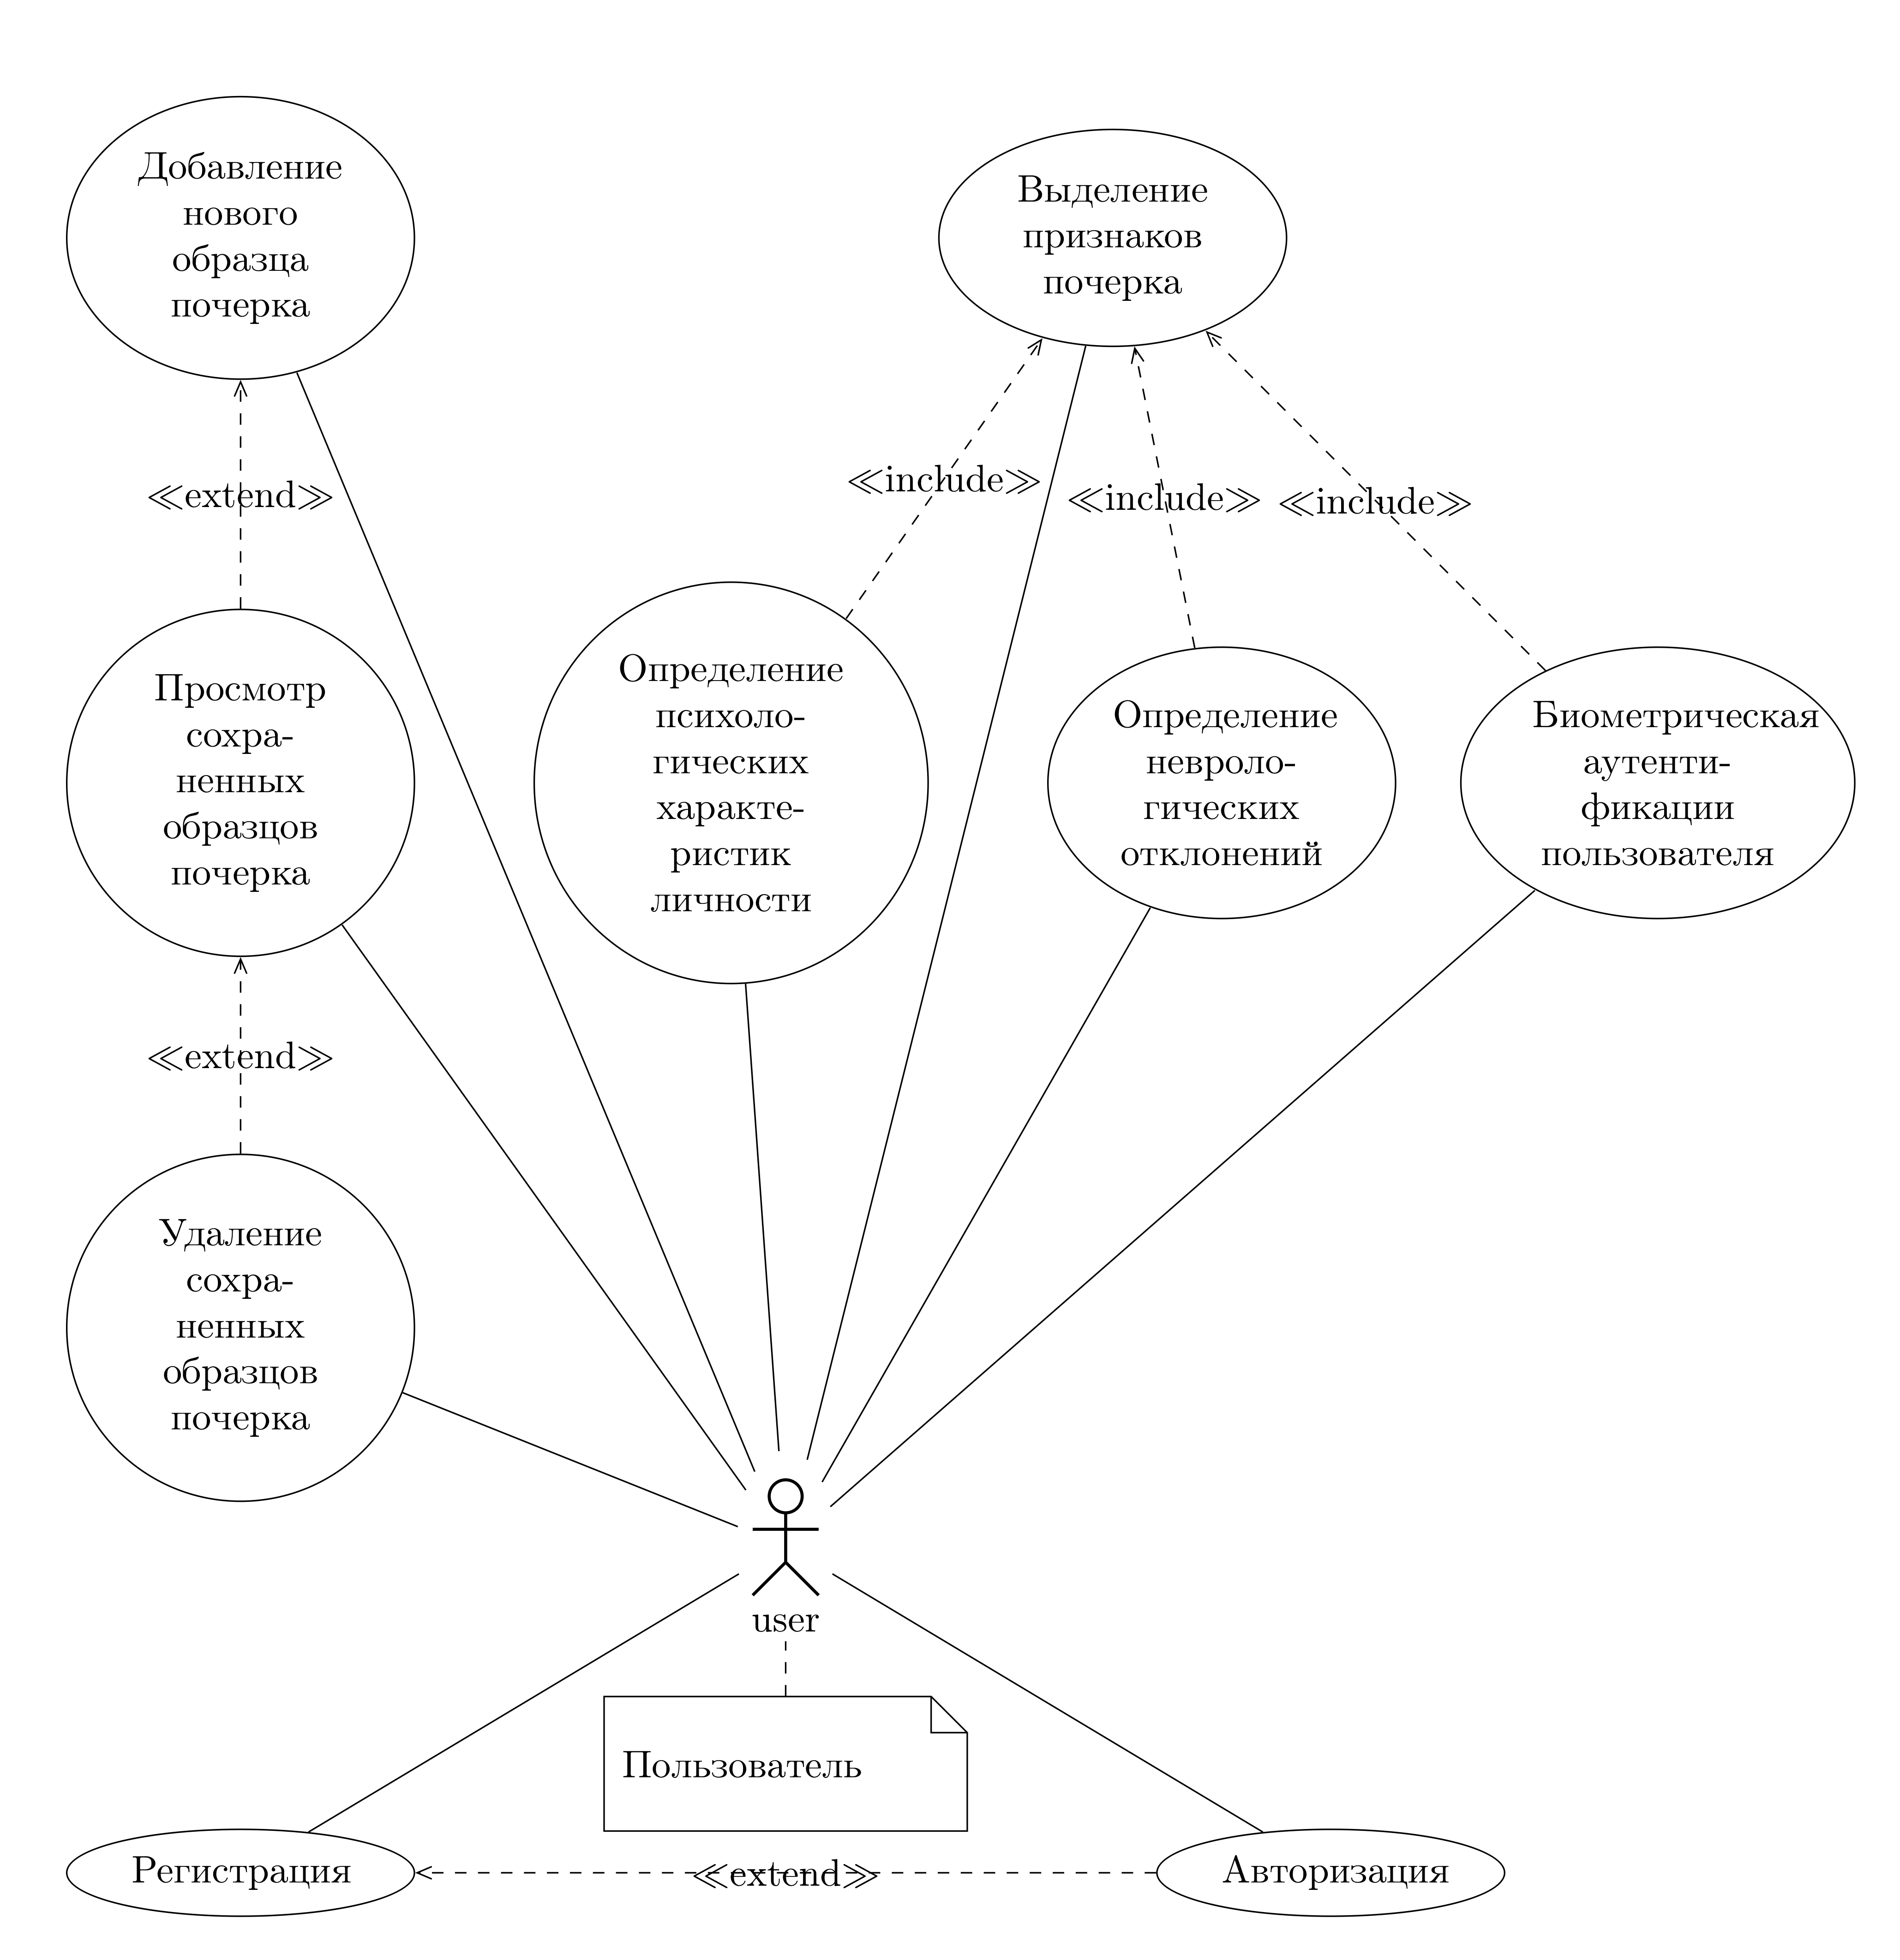
\includegraphics[scale=1]{figures/use_case.png}  
    \caption{Диаграмма вариантов использования}
  \label{fig:freg:usecase}
\end{figure}

\subsubsection{Подключение IP камер}
\begin{itemize}
	\item возможность подключится либо отключиться от камеры должна быть из пользовательского веб интерфейса;
	\item адреса добавленных IP камер должны сохранятся и при перезапуске сервера, сервер должен снова подключится к камерам;
	\item должна быть возможность добавить несколько IP камер;
	\item у каждой IP камеры кроме имени должен быть псевдоним, указываемый при подключении, который будет передаваться вместе с результатами распознавания в плагины.
\end{itemize}

\subsubsection{Загрузка изображений для распознавания}
\begin{itemize}
	\item возможность загрузить изображение на сервер для распознавания;
	\item поддержка форматов PNG и JPEG;
  \item должны быть показанны все шаги по распознаванию.
\end{itemize}

\subsubsection{Подключение плагинов}
\begin{itemize}
	\item плагины подключаются путем копирования dll файлов в директорию plugins, рядом с исполняемым файлом;
	\item для создания плагинов требуется используя библиотеку реализовать интерфейс обработчика результатов на платформе;
	\item плагины обрабатывают положительный и отрицательный результат.
\end{itemize}

\subsubsection{Процесс распознавания номеров}
\begin{itemize}
	\item сервер должен обрабатывать видеопоток от IP камер;
	\item при распознании результаты передаются подключенным плагинам;
	\item при команде открытия шлагбаума от оператора требуется передать плагинам отрицательный результат для обработки.
\end{itemize}

\subsubsection{Пользовательский интерфейс програмного средства}
\begin{itemize}
	\item пользовательский интерфейс должен быть Web страницей;
	\item должны поддерживаться Google Chrome и Firefox последних версий.
\end{itemize}

\subsubsection{Совместимость программного средства}
\begin{itemize}
  \item операционная система Windows не ниже 7 версии;
	\item CPU не менее 2.6 GGz 2 на обрабатываемый видеопоток;
  \item RAM 2 Gb + по 500 Mb на каждую обрабатываемую камеру.
\end{itemize}